\labeledsection{Inductive Logic Programming}{sec:inductive_logic}
\titledbox{Motivation}{
\begin{itemize}
    \item Previously, we talked about learning from examples (\linkterm{inductive learning}{supervised_learning})
    \item Main idea was $\leadsto$ constructing a \linkterm{function}{function} with the input-output behavior observed in the data
    \item The main method was searching for suitable \linkterm{hypothesis}{supervised_learning} in a \linkterm{hypothesis space}{supervised_learning}
    \item Every learning task begins from zero except we choose the \linkterm{hypothesis space}{supervised_learning}
\end{itemize}
}

\problembox{
We have to forget anything before we can learn something new
}

\ideabox{
Utilize prior knowledge about the world
}

\questionbox{How can we do that?}

\titledbox{Remember}{
\linkterm{examples}{supervised_learning} are composed of descriptions of the input sample and classifications
}

\ideabox{
Represent \linkterm{examples}{supervised_learning} and \linkterm{hypotheses}{supervised_learning} as logical formulae
}

\Example{
We can make \linkterm{attribute-based representation}{attribute_based_representations} using the language of First-Order Logic (\linkterm{$\text{PL}^1$}{pl1}). We can use \linkterm{predicate constants}{fol_sig_pl1} for Boolean attributes and classifications and \linkterm{function constants}{fol_sig_pl1} for other attributes.
}{}

\noindent\makebox[\textwidth]{%
\rule{0.25\textwidth}{0.4pt}\hfill
\textbf{Excursion : Recall - First-Order Logic}\hfill
\rule{0.25\textwidth}{0.4pt}%
}

\anondefinition{
\defemph{First-Order (Predicate) Logic} $\text{PL}^1$ is a \linkterm{formal system}{formal_system} extensively used in mathematics, philosophy, linguistics, and computer science. It combines \linkterm{$\text{PL}^0$}{def:pl0_as_ls} with the ability to quantify over \linkterm{individuals}{fol_sig}
}{pl1}

\anondefinition{
A \defemph{First-Order Signature} is a tuple $\Sigma := \tuple{\Sigma_1, \linkterm{\Sigma_0}{wff0_def}}$ where $\Sigma_1 := \Sigma^f \cup \Sigma^p \cup \Sigma^{sk}$:
\begin{itemize}
\item $\Sigma^f := \bigcup_{k \in \mathbb{N}} \Sigma_k^f$ of \textbf{function constants} (or \textbf{terms}), where members of $\Sigma_k^f$ denote the $k$-ary \linkterm{functions}{function} on \textbf{individuals}
\item $\Sigma^p := \bigcup_{k \in \mathbb{N}} \Sigma_k^p$ of \textbf{predicate constants}, where member of $\Sigma_k^p$ denote $k$-ary \linkterm{relations}{relation} among individuals
\item $\Sigma^{sk} := \bigcup_{k \in \mathbb{N}} \Sigma_k^{sk}$ of \textbf{Skolem constants} that act as witness constructors
\item All are \linkterm{pairwise disjoint}{pairwise_disjoint}, \linkterm{countable}{countable} \linkterm{sets}{def:set} of symbols for each $k \in \mathbb{N}$.
\end{itemize}
We also assume a \linkterm{set}{def:set} of \textbf{individual variables} $V_{\iota} := \set{X,Y,Z,\cdots}$ which we can quantify over them.
}{fol_sig_pl1}


\definition{\linkterm{$\text{PL}^1$}{pl1} Terms}{
The \linkterm{set}{def:set} $\text{wff}_{\iota}(\Sigma_1, V_{\iota})$ of \textbf{well-formed terms} over the signature $\Sigma_1$ and variables \linkterm{$V_{\iota}$}{fol_sig_pl1} is defined by the following \linkterm{grammar}{phrase_structure_grammar}:
\begin{align*}
f^k \quad &\in \quad \Sigma_k^f \cup \Sigma_k^{sk} \\
X \quad &\in \quad \linkterm{V_{\iota}}{fol_sig_pl1} \\ 
t \quad &::= \quad X \mid f^k(t_1, \cdots, t_k)
\end{align*}
}{terms_pl1}

\definition{\linkterm{$\text{PL}^1$}{pl1} Propositions}{
The \linkterm{set}{def:set} $\text{wff}_{\circ}(\Sigma_1, V_{\iota})$ of \textbf{well-formed formulae} over the signature $\Sigma_1$ and variables \linkterm{$V_{\iota}$}{fol_sig_pl1} is defined by the following \linkterm{grammar}{phrase_structure_grammar}:
\begin{align*}
p^k \quad &\in \quad \Sigma_k^p \\
t_i \quad &\in \quad \text{wff}_{\iota}(\Sigma_1, \linkterm{V_{\iota}}{fol_sig_pl1}) \\ 
X \quad &\in \quad \linkterm{V_{\iota}}{fol_sig_pl1} \\ 
A \quad &::= \quad p^k(t_1, \cdots, t_k) \mid \top \mid \neg A \mid A \land A \mid \forall X.A
\end{align*}
}{formulae_pl1}

\anondefinition{
The \textbf{universal quantifier} $\forall$ is a binding operator used to express $\forall X.A$, i.e. a \linkterm{formula}{formulae_pl1} $A$ holds for all possible values of an \linkterm{individual variable}{terms_pl1} $X \in$ \linkterm{$V_{\iota}$}{fol_sig_pl1}
}{forall}

\anondefinition{
The \textbf{existential quantifier} $\exists$ is a binding operator defined as an \textbf{abbreviation} for a negated universal statement: $\exists X.A :\equiv \neg (\forall X. \neg A)$. It allows us to express that at least one \linkterm{individual}{terms_pl1} satisfies the \linkterm{formula}{formulae_pl1} $A$.
}{exists}

\anondefinition{
A \linkterm{formula}{formulae} is called \textbf{atmoic} (or an \textbf{atom}) if it does not contain logical constants, otherwise, \textbf{complex}
}{atomic_formula}

\anondefinition{
Let $\mathcal{S} := \langle \mathcal{L}, \mathcal{M}, \vDash \rangle$ be a \linkterm{logical system}{logical_system}, $A \in \mathcal{L}$ a formula, $L$ a \textbf{label set}, and $\alpha \in L$ a \textbf{label}, then we call a \linkterm{pair}{cartesian_product} $\tuple{A, \alpha}$ a \textbf{labeled formula} and write it as $A^{\alpha}$. For a \linkterm{set}{def:set} $\Phi$ of \linkterm{propositions}{proposition} we use $\Phi^{\alpha} := \set{A^{\alpha} \mid A \in \Phi}$
}{labeled_formula}

\anondefinition{
Let $\mathcal{S} := \langle \mathcal{L}, \mathcal{M}, \vDash \rangle$ be a \linkterm{logical system}{logical_system}, $A \in \mathcal{L}$ is an \linkterm{atomic formula}{atomic_formula}, and $\alpha \in \set{T,F}$, then we call the \linkterm{labeled formula}{labeled_formula} $A^{\alpha}$ a \textbf{literal}.
}{literal}


\noindent\makebox[\textwidth]{%
\rule{0.3\textwidth}{0.4pt}\hfill
\textbf{End of Excursion}\hfill
\rule{0.3\textwidth}{0.4pt}%
}

\anondefinition{
\defemph{Logic-based inductive learning} tries to learn a \linkterm{hypothesis}{supervised_learning} $h$ that explains the \linkterm{classifications}{classifcation_regression} of the \linkterm{examples}{supervised_learning} given their \defemph{description}, i.e. $h, \mathcal{D} \sat \mathcal{C}$ (the \defemph{explanation constraint}), where:
\begin{itemize}
    \item $\mathcal{D}$ is the conjunction of the \defemph{descriptions}, and
    \item $\mathcal{C}$ is the conjunction of their \linkterm{classifications}{classifcation_regression}
\end{itemize}
}{logic_based_inductive_learning}

\commandnote{
The idea is that we solve the \linkterm{explanation constraint}{logic_based_inductive_learning} for $h$ where $h$ ranges over some \linkterm{hypothesis space}{supervised_learning}
}

\Example{
Remember \Exampleref{restaurant_example}:

\begin{tabular}{c||c|c|c|c|c|c|c|c|c|c||c}
\hline
 & \multicolumn{10}{c||}{\textbf{Attributes}} & \textbf{Target} \\ \cline{2-11}
\textbf{Example} & \textit{Alt} & \textit{Bar} & \textit{Fri} & \textit{Hun} & \textit{Pat} & \textit{Price} & \textit{Rain} & \textit{Res} & \textit{Type} & \textit{Est} & \textit{WillWait} \\ \hline\hline
$X_1$  & T & F & F & T & Some & \$\$\$ & F & T & French  & 0--10  & T \\ 
$X_2$  & T & F & F & T & Full & \$    & F & F & Thai    & 30--60 & F \\ 
$X_3$  & F & T & F & F & Some & \$    & F & F & Burger  & 0--10  & T \\ 
$X_4$  & T & F & T & T & Full & \$    & F & F & Thai    & 10--30 & T \\ 
$X_5$  & T & F & T & F & Full & \$\$\$ & F & T & French  & $>$60  & F \\ 
$X_6$  & F & T & F & T & Some & \$\$   & T & T & Italian & 0--10  & T \\ 
$X_7$  & F & T & F & F & None & \$    & T & F & Burger  & 0--10  & F \\ 
$X_8$  & F & F & F & T & Some & \$\$   & T & T & Thai    & 0--10  & T \\ 
$X_9$  & F & T & F & T & Full & \$    & T & F & Burger  & $>$60  & F \\ 
$X_{10}$ & T & T & T & T & Full & \$\$\$ & F & T & Italian & 10--30 & F \\ 
$X_{11}$ & F & F & F & F & None & \$    & F & F & Thai    & 0--10  & F \\ 
$X_{12}$ & T & T & T & T & Full & \$    & F & F & Burger  & 30--60 & T \\ \hline
\end{tabular}

\linkterm{descriptions}{logic_based_inductive_learning} are conjunctions of \linkterm{literals}{literal} built up from
\begin{itemize}
    \item \linkterm{predicates}{fol_sig_pl1} \texttt{Alt}, \texttt{Bar}, \texttt{Fri/Sat}, \texttt{Hun}, \texttt{Rain}, \texttt{Res}
    \item Equations about the \linkterm{functions}{fol_sig_pl1} \texttt{Pat}, \texttt{Price}, \texttt{Type}, \texttt{Est}
\end{itemize}
For instance, the first \linkterm{example}{supervised_learning} $X_1$ can be described as:
\[
\text{Alt}(X_1) \land \neg \text{Bar}(X_1) \land \neg \text{Fri/Sat}(X_1) \land \text{Hun}(X_1) \land
\text{Pat}(X_1) = \text{Some} \land \cdots
\]
The \linkterm{classification}{classifcation_regression} is given by the goal \linkterm{predicate}{fol_sig_pl1} \texttt{WillWait}, in this case $\text{WillWait}(X_1)$ or $\neg \text{WillWait}(X_1)$
}{}


\Example{
Remember the induced \linkterm{DT}{decision_trees} from \Exampleref{ex:learned_dt}:
\begin{center}
    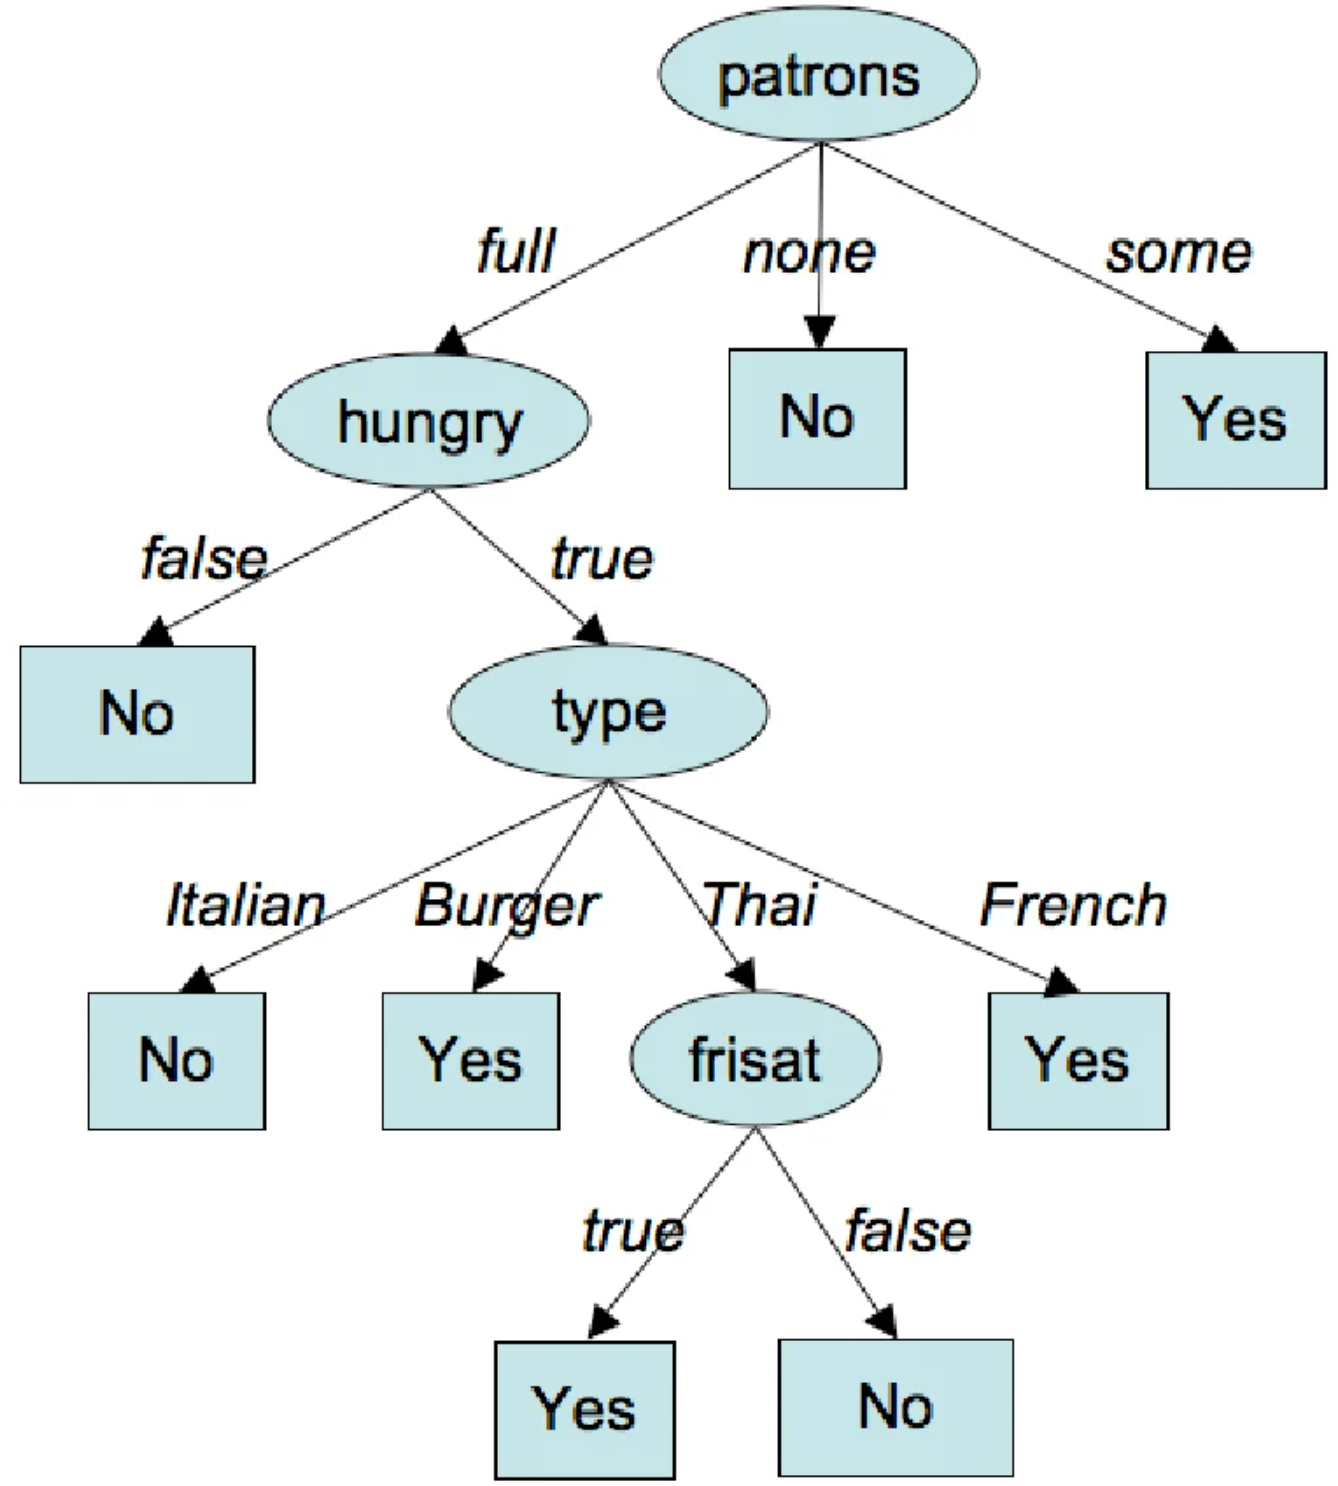
\includegraphics[width=0.3\linewidth]{images/restaurant_dtl.png}
\end{center}
This can be expressed as:
\begin{align*}
\forall r. \text{WillWait}(r) &\Leftrightarrow \text{Pat}(r, \text{Some}) \\ 
&\lor \text{Pat}(r, \text{Full}) \land \text{Hun}(r) \land \text{Type}(r, \text{French}) \\ 
&\lor \text{Pat}(r, \text{Full}) \land \text{Hun}(r) \land \text{Type}(r, \text{Thai}) \land \text{Fri/Sat}(r) \\ 
&\lor \text{Pat}(r, \text{Full}) \land \text{Hun}(r) \land \text{Type}(r, \text{Burger})
\end{align*}

\textbf{Method: }construct a disjunction of all the \linkterm{paths}{path_graph} from teh \linkterm{root}{tree} to the positive \linkterm{leaves}{tree} interpreted as conjunctions of the \linkterm{attributes}{attribute_based_representations} on the \linkterm{path}{path_graph}

\textbf{Note: }The equivalence takes care of positive and negative \linkterm{examples}{supervised_learning}
}{}

\observationbox{
We can represent unary \linkterm{function constants}{fol_sig_pl1} as binary \linkterm{predicate constants}{fol_sig_pl1} by shifting the output value into a second argument position, eliminating the need for the equality symbol ($=$):
\[
\text{Function}(x) = \text{value} \quad\leadsto\quad \text{Predicate}(x, \text{value})
\]
For example, $\text{Type}(X_1) = \text{French}$ becomes $\text{Type}(X_1, \text{French})$.
}

\titledbox{Machine Learning vs Humans}{
\begin{itemize}
    \item Standard machine learning algorithms starts from scratch. To learn a new concept, they require hundreds of thousands of examples because they have to figure out all the rules of the world from data alone.
    \item In contrast, humans can learn a general rule from a single example because we do not start from zero; we use what we already know about the world to fast-track our understanding.
\end{itemize}
}

\Example{\textbf{Caveman Zog}: 

If Zog sees someone put a fish on a stick over a fire and it tastes good, he doesn't need to try cooking a hundred different fish on a hundred different sticks to form a hypothesis. He instantly generalizes: “Food on a stick over fire cooks well.” He uses his prior understanding of fire, wood, and eating.
}{}

\Example{\textbf{The Brazilian}: 

If you meet one Brazilian and they speak Portuguese, you immediately assume most Brazilians speak Portuguese. You don't need a sample size of 10,000 citizens because your background knowledge already includes the concept of "national languages."
}{}

\Example{\textbf{Johanna and the Antibiotic}: 

Johanna knows nothing about the drug Proxadone, but she knows the doctor is an expert, an inflamed foot indicates a bacterial infection, and antibiotics kill bacteria. From observing one single prescription, she infers that Proxadone is effective against foot infections.
}{}

\problembox{
\linkterm{Supervised learning}{supervised_learning} cannot replicate this.

}

\questionbox{Why?}

\answerbox{
Standard algorithms fail here because they lack context. If you feed a standard algorithm a dataset with a single row containing $[\text{Patient\_ID}, \text{Inflamed\_Foot}, \text{Proxadone}] \Rightarrow [\text{Cured}]$, it cannot statistically justify generalizing this to all future patients. It sees it as an isolated statistical fluke or a correlation of size 1.
}

\solutionbox{
To bridge this gap, \linkterm{logic-based learning}{logic_based_inductive_learning} explicitely introduces \defemph{Background Knowledge} $\mathcal{B}$. Instead of searching for a \linkterm{hypothesis}{supervised_learning} $h$ based only on the \linkterm{descriptions}{logic_based_inductive_learning} $\mathcal{D}$ and \linkterm{classifications}{classifcation_regression} $\mathcal{C}$, the \linkterm{explanation constraint}{logic_based_inductive_learning} is upgraded to include what the system already knows.
\[
\mathcal{B} \land h \land \mathcal{D} \sat \mathcal{C}
\]
}


\titledbox{Cumulative Development}{
The ultimate goal is \defemph{cumulative learning}
\begin{itemize}
    \item We start with some prior knowledge
    \item We observe the world and learn a new rule/\linkterm{hypothesis}{supervised_learning} efficiently using that prior knowledge.
    \item This new \linkterm{hypothesis}{supervised_learning} is validated, becomes true, and is added back into our body of background knowledge $\mathcal{B}$
    \item For the next learning task, our $\mathcal{B}$ is now larger and richer, making the next round of learning even faster and more sophisticated
\end{itemize}
}

\anondefinition{
We call the body of knowledge accumulated by (a group of) \linkterm{agents}{def:agent} their \defemph{background knowledge}. It acts as \defemph{prior knowledge} in \linkterm{logic-based learning}{logic_based_inductive_learning} processes
}{bg_knowledge}

\begin{figure}[H]
    \centering
    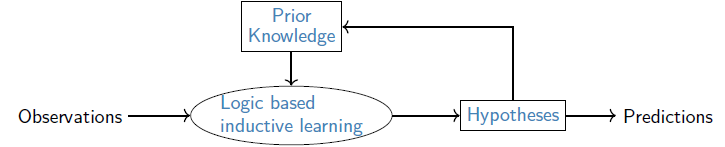
\includegraphics[width=0.5\linewidth]{images/logic_learning.png}  
\end{figure}

\anondefinition{
\defemph{Knowledge-based inductive learning (KBIL)} replaces the \linkterm{explanation constraint}{logic_based_inductive_learning} by the \defemph{KBIL constraint}:
\[
\mathcal{B} \land h \land \mathcal{D} \sat \mathcal{C}
\]
}{KBIL}

\centeredtitledbox{Remember \Defref{def:reasoning}}{
Deduction $\hat{=}$ knowledge extension
\Example{
\[
    \infer[D]{\text{wet\_street}}{\text{rains} \Rightarrow \text{wet\_street} \quad \text{rains}}
\]
}{}

Abduction $\hat{=}$ explanation
\Example{
\[
    \infer[A]{\text{rains}}{\text{rains} \Rightarrow \text{wet\_street} \quad \text{wet\_street}}
\]
}{}

Induction $\hat{=}$ learning general rules from \linkterm{examples}{supervised_learning}
\Example{
\[
    \infer[I]{\text{rains} \Rightarrow \text{wet\_street}}{\text{wet\_street} \quad \text{rains}}
\]
}{}
}

\anondefinition{
\defemph{Inductive Logic Programming (ILP)} is a \linkterm{logic-based inductive learning method}{logic_based_inductive_learning} that uses logic programming as a uniform representation for \linkterm{examples}{supervised_learning}, \linkterm{background knowledge}{bg_knowledge} and \linkterm{hypotheses}{supervised_learning}. Given an encoding of the known \linkterm{background knowledge}{bg_knowledge} and a \linkterm{set}{def:set} of \linkterm{examples}{supervised_learning} represented as logical knowledge base of facts, an \defemph{ILP} system will derive a hypothesized logic program which entails all the positive and none of the negative \linkterm{examples}{supervised_learning}
}{ILP}

\commandnote{
\linkterm{Prior knowledge}{bg_knowledge} plays two key roles:
\begin{itemize}
    \item The effective \linkterm{hypothesis space}{supervised_learning} is reduced to include only those theories that are consistent with what is already known
    \item \linkterm{Prior knowledge}{bg_knowledge} can be used to reduce the size of the \linkterm{hypothesis}{supervised_learning} explaining the observations $\leadsto$ smaller \linkterm{hypotheses}{supervised_learning} are easier to find
\end{itemize}
}

\observationbox{
\linkterm{ILP}{ILP} systems can formulate \linkterm{hypotheses}{supervised_learning} in \linkterm{First-Order Logic}{pl1}
}

\Example{
\textbf{Learning family relations from examples}

\begin{itemize}
    \item Observations are an extended family tree 
    \begin{itemize}
        \item \texttt{mother}, \texttt{father}, and \texttt{married} relations (binary predicates)
        \item \texttt{male} and \texttt{female} propoerties (unary predicates)
    \end{itemize}
    \item Target predicates: \texttt{grandparent}, \texttt{BrotherInLaw}, \texttt{Ancestor}
    \item The goal is to find a logical formula that serves as a \linkterm{definition}{definitions} of the target predicates
    \item Equivalently: A Prolog program that computes the value of the target predicate 
\end{itemize}
}{}

\Example{
\begin{figure}[H]
    \centering
    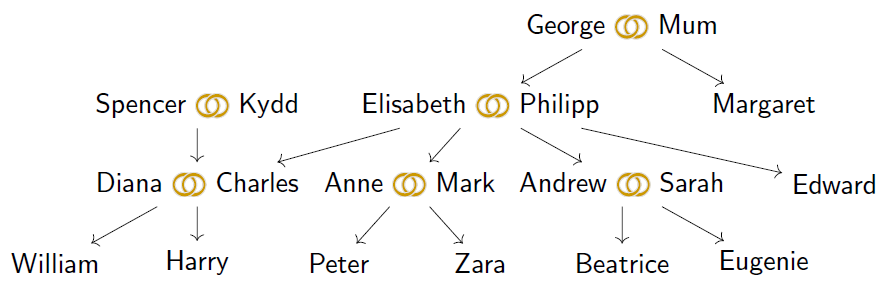
\includegraphics[width=0.5\linewidth]{images/family_tree.png}
\end{figure}
}{}

\linkterm{Descriptions}{logic_based_inductive_learning} include facts like
\begin{itemize}
    \item $\text{father}(\text{Philip}, \text{Charles})$
    \item $\text{mother}(\text{Mum}, \text{Margaret})$
    \item $\text{married}(\text{Diana}, \text{Charles})$
    \item $\text{male}(\text{Philip})$
    \item $\text{female}(\text{Beatrice})$
\end{itemize}

An analysis of the family tree yields a total of 24 positive instances for the \texttt{grandparent} predicate, categorized by lineage layer:

\begin{itemize}
    \item \textbf{Top-Generation Lineage (George \& Mum)}
    \begin{itemize}
        \item $\text{grandparent}(\text{George}, \text{Charles})$
        \item $\text{grandparent}(\text{George}, \text{Anne})$
        \item $\text{grandparent}(\text{George}, \text{Andrew})$
        \item $\text{grandparent}(\text{George}, \text{Edward})$
        \item $\text{grandparent}(\text{Mum}, \text{Charles})$
        \item $\text{grandparent}(\text{Mum}, \text{Anne})$
        \item $\text{grandparent}(\text{Mum}, \text{Andrew})$
        \item $\text{grandparent}(\text{Mum}, \text{Edward})$
    \end{itemize}

    \item \textbf{Central Royal Lineage (Elisabeth \& Philipp)}
    \begin{itemize}
        \item $\text{grandparent}(\text{Elisabeth}, \text{William})$
        \item $\text{grandparent}(\text{Elisabeth}, \text{Harry})$
        \item $\text{grandparent}(\text{Elisabeth}, \text{Peter})$
        \item $\text{grandparent}(\text{Elisabeth}, \text{Zara})$
        \item $\text{grandparent}(\text{Elisabeth}, \text{Beatrice})$
        \item $\text{grandparent}(\text{Elisabeth}, \text{Eugenie})$
        \item $\text{grandparent}(\text{Philipp}, \text{William})$
        \item $\text{grandparent}(\text{Philipp}, \text{Harry})$
        \item $\text{grandparent}(\text{Philipp}, \text{Peter})$
        \item $\text{grandparent}(\text{Philipp}, \text{Zara})$
        \item $\text{grandparent}(\text{Philipp}, \text{Beatrice})$
        \item $\text{grandparent}(\text{Philipp}, \text{Eugenie})$
    \end{itemize}

    \item \textbf{Maternal Lineage (Spencer \& Kydd)}
    \begin{itemize}
        \item $\text{grandparent}(\text{Spencer}, \text{William})$
        \item $\text{grandparent}(\text{Spencer}, \text{Harry})$
        \item $\text{grandparent}(\text{Kydd}, \text{William})$
        \item $\text{grandparent}(\text{Kydd}, \text{Harry})$
    \end{itemize}
\end{itemize}

\titledbox{Classification Data Split}{
We are currently trying to learn the \texttt{grandparent} rule, so our positive and negative training examples are populated with grandparent facts. For the \texttt{grandparent} relation in this problem instance, the dataset explicitly provides only $12$ positive examples alongside $376$ negative examples:
\begin{itemize}
    \item \textbf{Positive Examples:} e.g., $\text{grandparent}(\text{Mum}, \text{Charles})$
    \item \textbf{Negative Examples:} e.g., $\neg \text{grandparent}(\text{Mum}, \text{Harry})$
\end{itemize}
}

\observationbox{
While there are 24 biological grandparent pairs in the tree, we only need to specify 12 positive examples. The remaining 12 pairs can be completely inferred by the learner by utilizing the \texttt{married} relation present in our background knowledge base ($\mathcal{B}$).
}

\commandnote{
The classification dataset split is derived from the total possible pairwise combinations of individuals in the closed domain under a partial world view:
\begin{itemize}
    \item \textbf{Total Domain Size ($N$):} There are $20$ distinct individuals named in the family tree.
    \item \textbf{Total Relation Space ($N \times N$):} Evaluating every possible candidate pair for the binary predicate $\text{grandparent}(X, Y)$ yields $20 \times 20 = 400$ total possible permutations.
    \item \textbf{Negative Examples Calculation:} Out of the $388$ biologically non-positive pairs ($400 - 24$), we explicitly include $376$ as negative examples. The remaining $12$ true relationships are left completely unlabeled/unclassified to allow the system to infer them via background knowledge (e.g., using the \texttt{married} relation) without causing a logical contradiction.
\end{itemize}
}

\Example{
Without \linkterm{background knowledge}{bg_knowledge}, the system defines \texttt{grandparent} in terms of \texttt{mother} and \texttt{father}:
\[
\text{grandparent(x,y)} \Leftrightarrow (\exists z. \text{mother}(x,z) \land \text{mother}(z,y))
\lor 
(\exists z. \text{mother}(x,z) \land \text{father}(z,y)) \lor \cdots \lor     
(\exists z. \text{father}(x,z) \land \text{father}(z,y)) 
\]
}{}

\commandnote{
Standard \linkterm{attribute}{attribute_based_representations}-based algorithms (like \linkterm{DTs}{decision_trees}) are structurally incapable of learning relational concepts like $\text{grandparent}(X, Y)$.
}

\questionbox{Why?}

    Standard machine learning models expect each row in a dataset to represent a single, independent object. To learn a binary relation, the input "object" must be forced into an artificial tuple or pair, such as:
    \[
    O = \langle \text{Mum}, \text{Charles} \rangle
    \]
    
    Because a standard decision tree cannot look up other rows dynamically or link variables across features, we cannot create an abstract column like $\text{parent}(X, Z)$. Instead, we are forced to engineer hyper-specific, hardcoded Boolean attributes for each specific individual in the domain:
    \[
    \text{FirstElementIsMotherOfElisabeth}(O) \rightarrow \text{True}
    \]
    \[
    \text{SecondElementIsSonOfElisabeth}(O) \rightarrow \text{True}
    \]
    
    Lacking the capacity for variables, the induced decision tree cannot uncover the underlying transitivity rule. It simply memorizes the training instances, collapsing into a massive, flat disjunction ($\lor$) of specific lookups:
    \[
    \text{Grandparent}(O) \Leftrightarrow \left(\text{First}(O) = \text{Mum} \land \text{Second}(O) = \text{Charles}\right) \lor \left(\text{First}(O) = \text{George} \land \text{Second}(O) = \text{Anne}\right) \lor \dots
    \]


\observationbox{
\textbf{The Takeaway:} Attribute-based learning algorithms learn concepts based entirely on the static \defemph{properties of objects}. They are structurally blind to the \defemph{relations between objects}. To effectively learn relational predicates, the hypothesis language must support variables and quantification ($\forall, \exists$), requiring a transition to First-Order Logic via Inductive Logic Programming.
}